\section{Comparison}
Per comparare due opere si è deciso di usare la clusterizzazione \gls{fcm} in grado di dipendere meno da eventuale rumore, soprattutto perché la comparazione tra due opere farà leva sulle densità più ridotte e quindi il rumore potrebbe inquinare i risultati.

\noindent In questa sottosezione vedremo in dettaglio l'algoritmo per la comparazione tra opere e si vedrà un esempio di applicazione per indagare al meglio le sue caratteristiche.

\paragraph{Definizioni}
Come si è già accennato in \cref{chap:LiteratureReview}, servirà fornire una definizione di misura del cluster e di probabilità di appartenenza ad un cluster da parte di una distribuzione. Ad esempio per \gls{kmeans} la misura di un cluster è stata definita come:
\begin{equation*}
	\mu(c) = {\sqrt{\mathbb{E}_\mathcal{L}\left[\left\|x-c\right\|^2\middle|\mathcal{P}(x)=c\right]}\,}^{k} \approx {\sqrt{\frac{1}{\left|\{x:\mathcal{P}(x)=c\}\right|}\sum_{x:\mathcal{P}(x)=c}\left\|x-c\right\|^2}\,}^{k}
\end{equation*}
dove $k$ è la dimensione dello spazio dei dati, $\mathcal{P}$ è il predittore di \gls{kmeans}, $\mathcal{L}$ è la distribuzione fusa delle due distribuzioni, $c$ è il centroide.

\noindent Nel nostro caso non esiste un predittore poiché è stata definita una misura di appartenenza di ogni dato ad ogni cluster. Tuttavia si ricorda che \gls{fcm} nasce da una generalizzazione di \gls{kmeans} e che dunque si può riprendere la formula minimizzata dall'algoritmo \gls{em} (\cref{eq:loss})
\begin{definition}[misura di un cluster]
\label{def:cluster_measure}
	Applicando \gls{fcm} al data set $\mathcal{S}$ con pesi $w$, otteniamo la misura di appartenza $\mu$ e i centroidi $\mathcal{C}$. $\mu_x(c)$ sarà così l'appartenenza del dato $x\in\mathcal{S}$ al cluster $c\in\mathcal{C}$. Chiamato $k$ la dimensione dello spazio dove sono istanziati i dati di $\mathcal{S}$, si denota con $\mu(c)$ il peso del cluster $c$. Il peso sarà il volume della sfera cui raggio è la radice della media quadratica delle distanze del cluster:
	\begin{align}
		&u_{ij}^2 := w_i\mu_{x_i}(C_j)^2 \quad \text{or also} \quad u_{xc}^2 := w_x\mu_{x}(c)^2\\
		&\mu(c) := {\sqrt{\frac{\sum_{x\in\mathcal{S}} u_{xc}^2 \left\|x-c\right\|^2}{\sum_{x\in\mathcal{S}}u_{xc}^2}}\,}^k
		\label{eq:fcm_cluster_measure}
	\end{align}
\end{definition}

\noindent Definita la misura dei cluster sarà necessario poi parlare del peso di appartenenza della distribuzione $\mathcal{A}$ (o analogamente $\mathcal{B}$) ad un cluster $c$. In \gls{kmeans} questa appartenenza è stata facilmente attribuita alla probabilità: $\mathbb{P}_\mathcal{A}\left[\mathcal{P}(x)=c\right]$. Come già detto in precedenza, \gls{fcm} non propone un predittore, quindi bisognerà fornire una definizione più generale. In \gls{kmeans} si può riformulare la probabilità di appartenenza come segue:
\begin{equation*}
	\mathbb{P}_\mathcal{A}\left[\mathcal{P}(x)=c\right] = \int d\mu_\mathcal{A}(x) \delta_x(c) = \int d\mu_\mathcal{A}(x) \mu_x(c)^2 \approx \frac{1}{|A|}\sum_{x\in A} \mu_x(c)^2\\
\end{equation*}
Ne consegue la definizione per \gls{fcm}:
\begin{definition}[peso di un cluster]
\label{def:weightovercluster}
	Si denota con $\omega_A(c)$ il peso del set $A$ sul cluster $c$ ottenuto con \gls{fcm}.
	\begin{equation}
		\omega_A(c) := \frac{\sum_{x\in A} u_{xc}^2}{\sum_{x\in A}w_x}
	\end{equation}
\end{definition}

\noindent Ora bisognerà definire l'indice di Jaccard, obiettivo non semplice poiché nella logica fuzzy la cardinalità di un insieme non è definita come nella logica booleana, poiché l'appartenenza stessa non ha un valore di verità binario. Inoltre si fa notare che è possibile fornire una definizione dettagliata dell'indice di Jaccard che non dipende da quanto detto fino ad ora, vedendo i due valori moltiplicati di natura differente. Ad esempio, possiamo essere portati a pensare che
\[
|D_A \cup D_B| = \sum_c \mu(c)
\]
a giudicare da quanto detto in \cref{def:cluster_measure}, tuttavia questa definizione è molto scomoda dal momento che non ci suggerisce niente in merito a $|D_A \cap D_B|$. Trattiamo quindi questa uguaglianza come una coincidenza nel caso di \gls{kmeans} che mette d'accordo un'eventuale definizione dell'indice di Jaccard con la definizione dell'integrale approssimato con \gls{montecarlo}.

\noindent Quindi pensiamo a $D_A$ e $D_B$ come dizionari, ossia l'elenco dei centroidi che riguardano $A$ e $B$.
\begin{definition}(Indice di Jaccard)
	\label{def:Jaccard_fcm}
	Si definiscono le operazioni di unione e intersezione in logica fuzzy come segue:
	\begin{align*}
	\mu_c(D_A\cup D_B) = \max\{\mu_c(D_A),\mu_c(D_B)\} \\
	\mu_c(D_A\cap D_B) = \min\{\mu_c(D_A),\mu_c(D_B)\}
	\end{align*}
	e si definisce la cardinalità di un insieme $S$ come: $|S|:=\sum_c \mu_c(S)$

	\noindent L'appartenenza di un cluster $c$ al dizionario $D_A$ sarà così definita:
	\begin{equation}
		\mu_c(D_A) = \max_{x\in A}(u_{xc}^2)
	\end{equation}
	analogamente per $\mu_c(D_B)$.

	\noindent Per questa ragione la definizione di indice di Jaccard che ne segue sarà:
	\begin{equation}
		J_{D_A,D_B} := \frac{|D_A \cap D_B|}{|D_A \cup D_B|} = \frac{\sum_c \min\{\max_{x\in A}(u_{xc}^2),\max_{x\in B}(u_{xc}^2)\}}{\sum_c \max\{\max_{x\in A}(u_{xc}^2),\max_{x\in B}(u_{xc}^2)\}}
	\end{equation}
\end{definition}

\noindent \cref{def:weightovercluster,def:cluster_measure,def:Jaccard_fcm} sono sufficienti per formulare la distanza tra due campionamenti proposta a seguito di \gls{fcm}.


\paragraph{L'algoritmo}
L'algoritmo prevede inizialmente di applicare \gls{fcm} al set fuso di dati delle due opere, al fine definire la misura e la discretizzazione dello spazio delle tessere. Non sarà necessario aver memoria dei centroidi, sarà altresì utile poter calcolare:
\begin{itemize}
	\item $ \mu(c) = {\sqrt{\frac{\sum_{x\in\mathcal{S}} u_{xc}^2 \|x-c\|^2}{\sum_{x\in\mathcal{S}}u_{xc}^2}}\,}^k $
	\item $ \omega_A(c) = \frac{\sum_{x\in A} u_{xc}^2}{\sum_{x\in A}w_x} $ e analogamente $ \omega_B(c) = \frac{\sum_{x\in B} u_{xc}^2}{\sum_{x\in B}w_x} $
	\item $ J_{D_A, D_B} $ definito in \cref{def:Jaccard_fcm}
\end{itemize}
La distanza tra opere sarà così definita come:
\begin{equation}
\label{eq:fuzzy_distance}
	d_{\gls{fcm}}(A, B) = (1 + J_{D_A, D_B})^{-1}\frac{\sum_c \left(\frac{r(c)-1}{r(c)+1}\right)^2 \mu(c)}{\sum_c \mu(c)}
\end{equation}
dove $r(c)$ è il rapporto tra le densità ossia tra $\omega_A(c)$ e $\omega_B(c)$.

\noindent Qui di seguito è mostrata una semplice applicazione per un set sintetico di dati. Come fatto in \cref{chap:LiteratureReview} si generano dei dati in uno spazio bidimensionale e si clusterizzano con \gls{fcm} in $64$ cluster.

\noindent In \cref{fig:fused_data_2D_fcm} sono mostrati i dati usati, si tratta di normali gaussiane con una certa rappresentanza e del rumore uniforme. I due set, chiamati $A$ e $B$, sono stati poi fusi e clusterizzati con \gls{fcm} (in \cref{fig:fcm_2D_fcm} una rappresentazione). In \cref{fig:measure_data_2D_fcm} sono raffigurati i cluster con le rispettive rappresentabilità tra il set $A$ e $B$ attraverso una mappa di colori.

\newpage
\begin{figure}[H]
	\centering
	\begin{subfigure}{0.45\linewidth}
		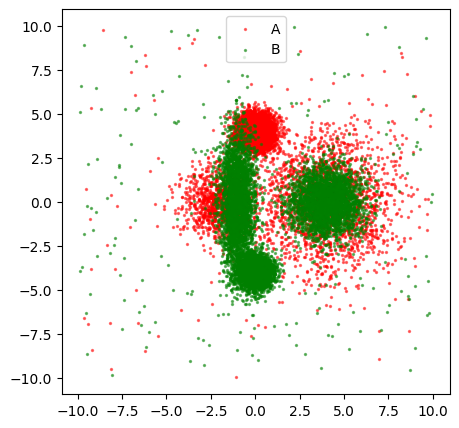
\includegraphics[width=\linewidth]{Figures/fused_data_2D_fcm.png}
		\caption[Application of fcm distance - fused data]{In figura sono mostrati i due set di immagini. \vspace{3.50em}}
		\label{fig:fused_data_2D_fcm}
	\end{subfigure}
	\hfill
	\begin{subfigure}{0.45\linewidth}
		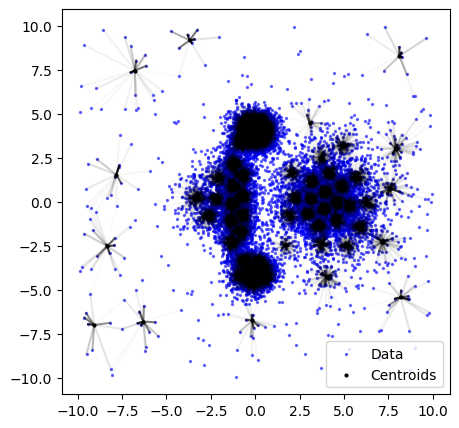
\includegraphics[width=\linewidth]{Figures/fcm_2D_fcm.png}
		\caption[Application of fcm distance - fcm application]{In figura è mostrata una clusterizzazione \gls{fcm} con $64$ centroidi, attraverso dei segmenti sono rappresentate le relazioni significative tra dati e cluster.}
		\label{fig:fcm_2D_fcm}
	\end{subfigure}
	\begin{subfigure}{\linewidth}
		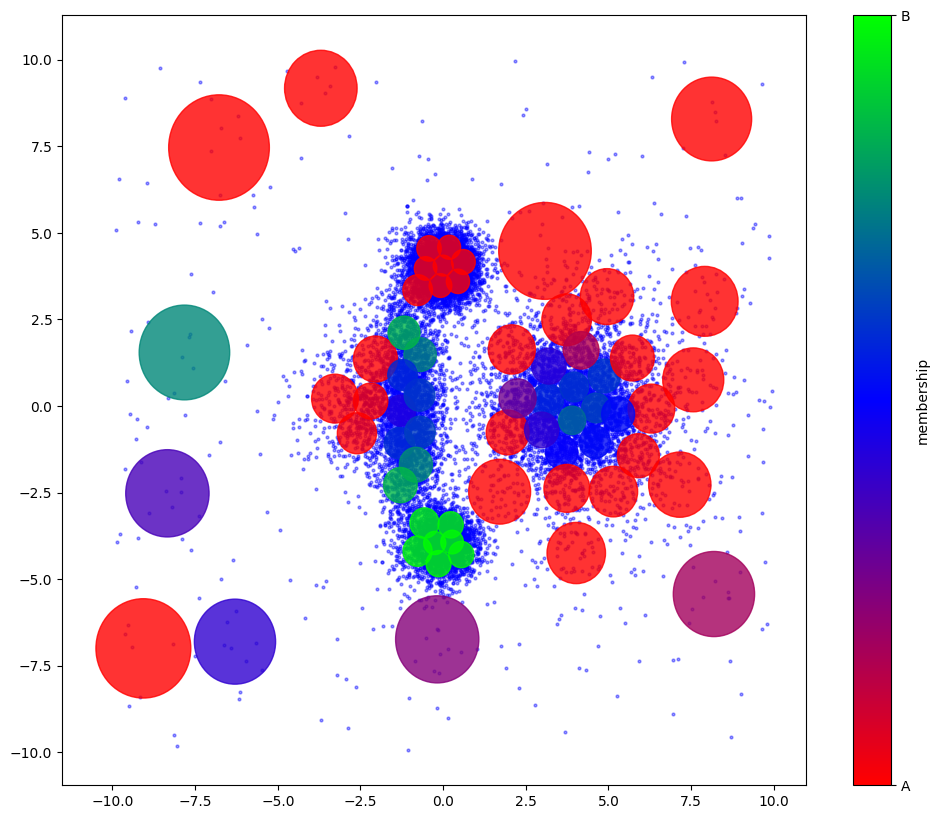
\includegraphics[width=\linewidth]{Figures/measure_2D_fcm.png}
		\caption[Application of fcm distance - discretisation]{In figura sono mostrati i cluster aventi un'area che copre la misura del cluster e un colore che ne indica la caratterizzazione, in particolare la scala di colori è mappata su $\frac{\omega_A-\omega_B}{\omega_A+\omega_B}$.}
		\label{fig:measure_data_2D_fcm}
	\end{subfigure}
\end{figure}

\newpage
\noindent Calcoliamo l'indice di Jaccard:
\begin{itemize}
	\item $ |D_A| = 53.17 $ e $ |D_B| = 52.26 $
	\item $ |D_A\cap D_B| = 43.91 $ e $ |D_A \cup D_B| = 61.53 $
	\item $ J_{D_A,D_B} = 0.71 $
\end{itemize}
Stimo l'integrale e di conseguenza la distanza tra le distribuzioni:
\begin{itemize}
	\item $ \frac{\sum_c \left(\frac{r(c)-1}{r(c)+1}\right)^2 \mu(c)}{\sum_c \mu(c)} = 0.31 $
	\item $ (1 + J_{D_A, D_B})^{-1} = 0.58 $
	\item $ d(A,B) = 0.18 $
\end{itemize}
Osserviamo che il risultato pur essendo in presenza di rumore non è molto dissimile dal risultato ottenuto con \gls{kmeans} in assenza di rumore (vedere \cref{tab:kmeans_tessellation_comparison}). Un altro esempio è con $256$ nodi dove la distanza sarà $0.38$ quindi ancora una volta non ci sono problemi legati al rumore.

\noindent Verifichiamo la potenzialità di \gls{fcm} esaminando le distanze computate da \gls{kmeans} in presenza di rumore:
\begin{itemize}
	\item[$64$:] la distanza stimata è $0.12$ contro la precedente $0.30$.
	\item[$256$:] la distanza stimata è $0.23$ contro la precedente $0.34$
\end{itemize}
La riduzione della distanza è un fenomeno atteso, poiché il rumore è identico per entrambi i campionamenti rendendoli quindi più simili. \gls{fcm} può lievemente pulire i set dal rumore e quindi avere una stima più precisa.

\paragraph{\gls{gpu}}
%L'algoritmo presentato è una soluzione sequenziale per l'estrazione delle tessere. Esso lavora iterando attraverso le righe e le colonne dell'immagine, estrae le tessere di dimensioni $N \times N$ e le inserisce in una lista. Tuttavia, questo approccio ha un costo computazionale pari a $O(hwN^2)$.\\
\noindent The \cref{alg:MembershipUpdateSafe} shown is a sequential solution for \gls{fcm}. It works by iterating through the data and centroids to compute the membership matrix. However, this approach has a computational cost of $O(NCk)$.

%Per migliorare l'efficienza computazionale, si può ricorrere all'utilizzo del boost della GPU (General Purpose Graphics Processing Unit). Questo genere di operazioni è noto come GPGPU (General-Purpose computing on Graphics Processing Units). Sfruttare la potenza di calcolo parallelo offerta dalle GPU può notevolmente accelerare il processo di estrazione delle tessere.
\noindent To improve computational efficiency, the use of \gls{gpu} \gls{boost}ing can be employed. This kind of operation is known as \gls{gpgpu}. Exploiting the parallel computing power offered by a \gls{gpu} can greatly accelerate the process of comparison.

%La \gls{gpu}, o unità di elaborazione grafica, è un componente elettronico presente in ogni computer, in grado di eseguire un grande numero di operazioni in parallelo. Originariamente concepita per gestire l'interfaccia grafica nei videogiochi, la \gls{gpu} si trova tipicamente nelle schede grafiche, dove è in grado di visualizzare miliardi di pixel sullo schermo di ogni computer a velocità che la \gls{cpu} non può raggiungere.\\
\noindent The \gls{gpu} is an electronic component present in every computer, able to perform a large number of operations in parallel. Originally designed to handle the graphical interface in video games, the \gls{gpu} is capable of handling billions of pixels on any computer screen at speeds that the \gls{cpu} cannot achieve.

%Questo processore è costituito da migliaia di thread, organizzati gerarchicamente a livello hardware per massimizzarne le prestazioni:
%\begin{enumerate}[label=\roman*.]
%\item \gls{sm}: Esegue un kernel e consiste di numerosi warp;
%\item \gls{warp}: Esegue il kernel del suo stream e possiede una memoria condivisa tra i suoi thread, di solito $32$;
%\item \gls{thread}: Esegue il kernel del suo warp sincronizzandosi con gli altri \gls{thread} dello stesso \gls{warp} e possiede una propria memoria riservata nei suoi registri.
%\end{enumerate}
\noindent This processor is made up of thousands of threads, organised hierarchically at the hardware level to maximise performance:
\begin{enumerate}[label=\roman*.]
\item \gls{sm}: Runs a kernel and consists of numerous \gls{warp}s;
\item \gls{warp}: Runs the kernel of its stream and has shared memory between its threads, usually $32$;
\item \gls{thread}: Executes the kernel of its warp by synchronising with the other \gls{thread}s of the same \gls{warp} and has its own reserved memory in its registers.
\end{enumerate}
%La memoria alla quale può accedere una \gls{gpu} è suddivisa in diverse categorie, tra cui la memoria \textit{global}, \textit{shared}, \textit{cache} e \textit{register}. L'accesso a queste memorie da parte dei \gls{thread} del processore dipende dalla gerarchia dei \gls{thread} stessi. Ad esempio, la memoria \textit{global} è accessibile da ogni \gls{thread}, mentre la memoria \textit{shared} è accessibile solo dai \gls{thread} appartenenti allo stesso \gls{warp}.\\
\noindent The memory that a \gls{gpu} can access is divided into different categories, namely \textit{global}, \textit{shared}, \textit{cache} and \textit{register} memory. Access to these memories by the processor's \gls{thread}s depends on the hierarchy of the \gls{thread}s themselves. For example, the \textit{global} memory is accessible by every \gls{thread}, while the \textit{shared} memory is only accessible by \gls{thread}s in the same \gls{warp}.

%In un computer di alta fascia, è comune trovare schede video dotate di $14$ \gls{sm}, ognuno dei quali contiene $1024$ \gls{thread} suddivisi in $32$ \gls{warp}. Questo totale di $14336$ \gls{thread} può eseguire in parallelo lo stesso identico codice, consentendo un'elaborazione estremamente veloce delle immagini e di altre operazioni che richiedono un alto grado di parallelismo.\\
\noindent In a high-end computer, it is common to find a \gls{gpu} equipped with $14$ \gls{sm}, each of which contains $1024$ \gls{thread}s divided into $32$ \gls{warp}s. This total of $14336$ \gls{thread}s can execute the exact same code in parallel, permitting extremely fast processing of images and other operations requiring a high degree of parallelism.

%A partire dagli anni $2000$, l'uso delle \gls{gpu} si è esteso al campo del calcolo scientifico, introducendo importati concetti come la scalabilità e l'\gls{hpc}. Dal $2020$, sono disponibili sul mercato \gls{gpu} dedicate alle operazioni di intelligenza artificiale.\\
\noindent Since the $2000$s, the use of \gls{gpu} has extended to the field of scientific computing, introducing important concepts such as scalability and \gls{hpc}. Since $2020$, dedicated \gls{gpu} are available on the market for artificial intelligence operations.

%In \gls{Python}, esistono framework utili per l'utilizzo delle \gls{gpu}, come \textit{torch} e \textit{TensorFlow}, ampiamente impiegati nell'ambito della computer vision. Tuttavia, anche linguaggi come il \verb"C++" offrono dialetti che consentono di sfruttare queste potenti unità di calcolo. In questo contesto, si userà il dialetto CUDA.\\
\noindent In \gls{Python}, there are useful frameworks for the utilisation of \gls{gpu}, such as \textit{torch} and \textit{TensorFlow}, which are widely employed in the field of computer vision. However, also languages such as \verb "C++" offer dialects that allow these powerful computing units to be exploited. In this paper, the \gls{cuda} dialect will be used.
\footnote{for more details about GPU architecture, see\newline\url{https://researchcomputing.princeton.edu/support/knowledge-base/gpu-computing}}
\footnote{for more details about \gls{cuda} language, see\newline\url{https://docs.nvidia.com/cuda/}}

\bigskip
The integration of \gls{gpgpu} techniques would allow the workload to be distributed over several cores of the \gls{gpu}, thus reducing the time needed for clustering operations. This method is particularly advantageous when handling large amounts of data, as the \gls{gpu} can perform many operations in parallel, speed up computation to be $2000$ times faster than the \gls{cpu} could have done.

\noindent The sum of $N$ numbers can be performed in with computational cost $O(log(N))$. This is because in parallel the \gls{gpu} threads sum one half of the vector over another at the same instant and then repeat until they get a single component that will have only one number. This operation is called \textit{reduction} and we can see it in the \cref{alg:gpu_reduction}. This is just one detail of how the \gls{gpu} can reduce the asymptotic computational cost of an algorithm. Suffice it to say that thanks to reductions and strong parallelism, it is possible to multiply two $N\times K$ and $K\times M$ matrices with cost $O(log(K))$ instead of $O(NMK)$. In clustering many operations can be parallelised and \gls{fcm} in particular requires many sums and linear operations.

\noindent The limitations of \gls{gpu} are not only related to the execution of the same operations on all threads, but also to the nature of these operations. Normally, an instruction takes much longer to be executed by a \gls{gpu} than by a \gls{cpu}. Arithmetic instructions are the most efficient, while the use of conditions tends to be avoided.

\begin{algorithm}
\caption{Parallel algorithm sum reduction}
\begin{algorithmic}[1]
\Procedure{Kernel $\textnormal{i}$, SumReduction}{$\textnormal{v}$,$\textnormal{N}$}
    \State Let $S$ a shared vector with $2^k \geq N$ component
    \State $S[\textnormal{i}] \gets \textnormal{v}[\textnormal{i}]$ if $\textnormal{i}<\textnormal{N}$ else $0$
    \For{$L \gets 2^{k}/2,2^{k}/4,\dots,1$}
        \If{$\textnormal{i} < L$}
            \State $S[\textnormal{i}] \gets S[\textnormal{i}] + S[\textnormal{i}+L]$
        \EndIf
        \State require synchronisation between threads
    \EndFor
\EndProcedure
\label{alg:gpu_reduction}
\end{algorithmic}
\end{algorithm}

\begin{figure}[h]
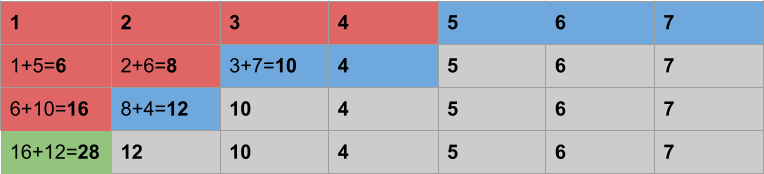
\includegraphics[width=\linewidth]{Figures/example_gpu_reduction.png}
\caption{We want to calculate the sum of the values in the first row. The idea is to divide the vector into $2$ regions, sum the components, and repeat over the new vector with half the size of the previous vector.}
\end{figure}
